\documentclass[conference]{IEEEtran}
\IEEEoverridecommandlockouts
% The preceding line is only needed to identify funding in the first footnote. If that is unneeded, please comment it out.
\usepackage{cite}
\usepackage{amsmath,amssymb,amsfonts}
%\theoremstyle{remark}
%\newtheorem{problem}{Problem}
\newtheorem{problem}{Problem}
\usepackage{algorithmic}
\usepackage{graphicx}
\usepackage{textcomp}
\usepackage{xcolor}
\def\BibTeX{{\rm B\kern-.05em{\sc i\kern-.025em b}\kern-.08em
    T\kern-.1667em\lower.7ex\hbox{E}\kern-.125emX}}
\begin{document}

\title{Missing Data Completion for Telco localization by Adversarial Learning\\
{\footnotesize \textsuperscript{}}
}

\author{\IEEEauthorblockN{Jinhua Lv}
\IEEEauthorblockA{\textit{Dept. of Software Engineering} \\
\textit{Tongji University}\\
Shanghai, China \\
jhlv@tongji.edu.cn}
\and
\IEEEauthorblockN{Weixiong Rao}
\IEEEauthorblockA{\textit{Dept. of Software Engineering} \\
\textit{Tongji University}\\
Shanghai, China \\
wxrao@tongji.edu.cn}
}

\maketitle

\begin{abstract}
This document is a model and instructions for \LaTeX.\\
This document is a model and instructions for \LaTeX.\\
This document is a model and instructions for \LaTeX.\\
This document is a model and instructions for \LaTeX.\\
This document is a model and instructions for \LaTeX.\\
This document is a model and instructions for \LaTeX.\\
This document is a model and instructions for \LaTeX.\\
This document is a model and instructions for \LaTeX.\\
This document is a model and instructions for \LaTeX.\\
This document is a model and instructions for \LaTeX.\\
This document is a model and instructions for \LaTeX.\\
This document is a model and instructions for \LaTeX.\\
This document is a model and instructions for \LaTeX.\\
This document is a model and instructions for \LaTeX.\\
This document is a model and instructions for \LaTeX.\\
This document is a model and instructions for \LaTeX.\\
This document is a model and instructions for \LaTeX.\\
\end{abstract}

\begin{IEEEkeywords}
component, formatting, style, styling, insert
\end{IEEEkeywords}
\section{Introduction}
Recent years witnessed the rapid spreading of cellular networks and pervasive mobile devices (MDs). The telecommunication (Telco) data, as trace of MDs in cellular networks, has many important applications for Telco operators, e.g., city-scale Telco localization \cite{DBLP:conf/cikm/ZhuLYZZGDRZ16}, churn prediction of subscribers \cite{DBLP:conf/sigmod/HuangZYDLND0Z15} and user experience assessment \cite{DBLP:journals/tist/LuoZYDY16}. In particular, as an important complementary technique of GPS, Telco localization is aimed at recovering mobility patterns of MDs at fine grained level (e.g., 20 meters). Unlike the call detail records (CDRs), Telco localization techniques mainly focus on measurement records (MRs), which measures radio signal strengths (RSSIs) between MD and its connected cells in Telco networks. In the past years, a plenty of Telco localization methods have been proposed to improve the performance under challenging city environment \cite{DBLP:conf/icc/IbrahimY11, DBLP:conf/icc/HaraAYDZ11,DBLP:journals/tvt/IbrahimY12,DBLP:conf/infocom/RayDM16,DBLP:conf/infocom/MargoliesBBDJUV17}.

However, these localization models are suffering from missing signal strength (RSSI) values. Zhu \cite{DBLP:conf/cikm/ZhuLYZZGDRZ16} found that nearly 50\% of real world MR records have RSSI with only 1 or 2 cells. Ray \cite{DBLP:conf/infocom/RayDM16} proposed a localization model based on that RSSI values from neighboring cells are all missing. The missing data problem significantly deteriorates the performance of Telco localization. There are two main reasons of missing values in MR records. One is that the mobile phones do not provide API to access neighboring cells. The other is that the RSSI is lost, due to communication failure or data corruption. Consequently, it is desired to develop a methodology with high completion performance to estimate the missing data.

%State-of-the-art data completion algorithms can be classified into two categories: statistical based methods and machine learning based methods. The statistical methods include mean imputation and regression models \cite{DBLP:journals/technometrics/Lazar03a}. The machine learning based methods build a predictive model to learn the internal mappings of data. These methods include algorithms based on K-nearest neighbor \cite{DBLP:journals/bioinformatics/TroyanskayaCSBHTBA01}, matrix completion \cite{DBLP:journals/jmlr/MazumderHT10}, Expectation Maximization \cite{DBLP:journals/nca/Garcia-LaencinaSF10} and deep neural networks such as denoising autoencoder (DAE) \cite{DBLP:conf/pakdd/GondaraW18}. However, the current machine learning based models have several drawbacks. For instance, 

State-of-the-art data completion algorithms can be classified into two categories: discriminative methods and generative methods. The discriminative models maximize the conditional probability of missing components given observed components. These methods include KNN \cite{DBLP:journals/bioinformatics/TroyanskayaCSBHTBA01}, MICE\cite{buuren2010mice} and matrix completion \cite{DBLP:journals/jmlr/MazumderHT10}. The generative methods maximize the joint probability of both observed and missing components, such as algorithms based on Expectation Maximization \cite{DBLP:journals/nca/Garcia-LaencinaSF10} and deep learning (e.g., denoising autoencoder (DAE)) \cite{DBLP:conf/icml/VincentLBM08,DBLP:conf/pakdd/GondaraW18}. However, there are two main challenges to directly apply existing data completion methods into our scenario. 1) \emph{Complex interactions of MR data}: Due to complicated Telco operation design \cite{DBLP:conf/infocom/MargoliesBBDJUV17}, the internal relationship of MR data is sophisticated and nonlinear. 2) \emph{Noisy signal strength}: The challenging RF propagation phenomena (e.g., multipath and non-line-of-sight) causes noise signal strength values. Noise caused by such fluctuation can hurt the inference of missing RSSI. Existing methods with shadow capability can not capture the distribution of MR data well. Besides, by retrieving locations from location-based services, the position labels is available in training data. However, such labels are not accessible in the testing phase. It is non-trivial to incorporate the position labels of training data into missing data completion.

%Besides, there is a major difference in our problem. The missing MR data to complete is collected without location labels (e.g., GPS coordinates) due to GPS issues \cite{DBLP:conf/mdm/ZhangRYZY17}. However, by retrieving locations from location-based services, it is available in historical collected MR data \cite{DBLP:journals/imwut/HuangLWCXZ17}. How to exploit these labels to help the generation of missing RSSI remains challenging.

With recent breakthroughs in deep learning, Generative Adversarial Nets (GANs), as a powerful technique for generative modelling, has shown impressive results in realistic data generation \cite{DBLP:conf/nips/GoodfellowPMXWOCB14,DBLP:conf/cvpr/LedigTHCCAATTWS17}. The GANs plays a game between two networks: a generator that produces completed MR data given MR missing data and a discriminator that produces probability distribution between the completed and real data \cite{DBLP:conf/nips/GoodfellowPMXWOCB14}. Compared with traditional machine learning models, the competing process between two networks are better at learning sophisticated internal correlation of data.

To this end, we propose TelcoGAN that built upon GANs to address the MR missing data problem. TelcoGAN takes advantage of available GPS location labels in training data set (e.g., retrieving location corrdinates from location-based services \cite{DBLP:journals/imwut/HuangLWCXZ17}), to stabilize the training process and lead to better completion performance. Our research makes two main contributions:

\begin{itemize}
  \item We propose TelcoGAN which cooperates a \emph{serving-centric space} and a \emph{localizer network} to produce high quality complete MR data. The serving-centric space component helps to learn the internal correlation of MR. The localizer network utilizes available GPS location labels to guide the adversarial process towards better results. In addition, we adopt a hybrid loss trick which combines mean squared loss and adversarial loss to further improve the performance.
  \item Evaluations on two real-world MR data sets show that our model achieves better performance than state-of-arts and the model trained on a spatial domain can improve the performance of another one.
\end{itemize}

The rest of this paper is organized as follows. Section II gives preliminary background and some related works. In Section III, we describe the technical design of TelcoGAN in detail. After that, we conduct extensive experiments in Section IV and review some related work in Section V. Finally, we conclude in Section VI.

Table  summarizes the main symbols and associated meanings used in this paper. 
\section{Preliminaries}
In this section, we first give a detailed description of MR data and the problem definition, next illustrate the solution overview, and finally give the basic of GANs \cite{DBLP:conf/nips/GoodfellowPMXWOCB14}.

\subsection{Data Description and Problem Definition}
Telco localization techniques mostly focus on MR data, which are generated when MDs connect to nearby cell towers in Telco networks. Generally, the MR data can be categorized into two aspects: (1) connected cells data including cell ids, cell locations; (2) continuous signal strength data, such as RSRP, RSSI. Table \ref{tab:mr} shows an example of MR record in 4G LTE network. A piece of MR record contains up to 6 nearby cells (\textbf{eNodeBID} and \textbf{CellID}) and radio signal strength indicators (RSSI) for each. Besides, it also marks a user ID (\textbf{IMSI}: International Mobile Subscriber identification Number) and connection time stamp (\textbf{MRTime}). Normally, Telco networks set one of the nearby cells as serving cell to provide data services or communication for the connected device. The serving cell is highlighted as \textbf{Serving\_eNodeBID} and \textbf{Serving\_CellID}, the same as the fist connected cell (\textbf{eNodeBID\_1} and \textbf{CellID\_1}).

%For the rest of this paper, a MR record and associated GPS label are denoted by $m$ and $l$ respectively. For a MR record $m$, it consists of cell id vector $c$, cell coordinate vector $d$ and RSSI vector $r$ with equal length as 6. Note that to protect privacy of involved users, we delete \textbf{IMSI} to reduce risk.

\begin{table}\scriptsize
\caption{An example of 4G LTE MR record}\label{tab:mr}
  \centering
  \begin{tabular}{|l|l||l|l|}
  \hline
  \textbf{Field}    & \textbf{Value}                 & \textbf{Field}    & \textbf{Value}   \\ \hline \hline
  MRTime            & \textbf{2017/5/31 14:12:06}    & IMSI              & \textbf{***012}  \\ \hline
  Serving\_eNodeBID & \textbf{99129}                 & Serving\_CellID   & \textbf{1}       \\ \hline
  eNodeBID\_1       & \textbf{99129}                 & CellID\_1         & \textbf{1}       \\ \hline
  RSRP\_1           & \textbf{-93.26}                & RSSI\_1           & \textbf{-67.18}  \\ \hline
  ...               & ...                            & ...               & ...              \\ \hline
  eNodeBID\_6       & \textbf{99145}                 & CellID\_6         & \textbf{5}       \\ \hline
  RSRP\_6           & \textbf{-90.02}                & RSSI\_6           & \textbf{-50.92}  \\ \hline
  \end{tabular}
\end{table}

%The MR missing data problem refers to missing of RSSI from neighboring cells. We assume that RSSI from any neighboring cell can be missing randomly (i.e., from $r_2$ to $r_6$). In addition, the binary vector $b=\{b_i\}_{i=1}^6$ taken values in $\{0, 1\}$ indicates which part of RSSI vector $r$ could be lost. Thus, an incomplete RSSI vector $\hat{r}$ can be defined as follow:
%
%\begin{equation}\label{eq:rssi}
%\hat{r_i}=\left\{
%\begin{aligned}
%&r_i, & \text{if}\enspace b_i=1 \\
%&nan,  & \text{otherwise}
%\end{aligned}
%\right.
%\end{equation}

%Note that we can recover binary vector $b$ from $\hat{r}$.

%The detail of the problem studied in this paper is described in Problem \ref{prob:miss}.

\begin{problem}\label{prob:miss}
  \textbf{[Telco Missing Data Completion]}: For a MR record with missing RSSI, Telco missing data completion problem is to recover a MR record with complete RSSI.
\end{problem}

\subsection{Solution Overview}


\subsection{Basic of GANs}
The key of Generative Adversarial Nets (GANs) \cite{DBLP:conf/nips/GoodfellowPMXWOCB14} is to play a competing game between two networks. The generator network $G$ takes noise vector $z$ as input and generates fake data. The discriminator network $D$ takes a data sample (real/generated) as input and try to classify the sample accurately. In contrast, the generator $G$ try to generate realistic data to fool discriminator $D$. Hence, the two networks $G$ and $D$ play a minimax game which can be formulated as:

\begin{equation}\label{eq:gan}
  \min\limits_G \max\limits_D \mathbb{E}_{\textbf{x}\sim p(\textbf{x})}[\log D(\textbf{x})]+\mathbb{E}_{\textbf{z}\sim p( \textbf{z})}[\log(1-D(G(\textbf{z})))]
\end{equation}

where $p(\textbf{x})$ denotes real data distribution, $p(\textbf{z})$ is noise distribution such as the uniform distribution or the normal distribution. The two networks are trained iteratively towards the optimization of objective function \ref{eq:gan}.

However, the unstable training process makes GANs hard to train. It has been shown in previous work \cite{DBLP:conf/icml/OdenaOS17} that the label information can help stabilize training, leading to improved quality of generated data. The auxiliary classification procedure is employed to help discriminator distinguish input samples from different label categories. A most recent work on multi-modality data completion employs the auxiliary label information and verifies the improvement \cite{DBLP:conf/kdd/CaiWGSJ18}. The proposed classification loss is described as follows:

\begin{equation}\label{eq:multi}
  L_{CLS}(x, y, l)=L_{CE}(D(x,y),\ell)
\end{equation}

where $x$, $y$ and $l$ denote observed variables, missing variables and associated label respectively. The discriminator is trained to minimize the classification loss of data samples, and meanwhile distinguish data samples (real/generated).

Inspired by the above methodologies, we propose our TelcoGAN model by adopting a deep localization model in a unified generative adversarial network, utilizing the available GPS label information in training data.

\section{TelcoGAN Model}
In this section, we introduce our TelcoGAN model for Telco missing data completion. The descriptions are separated into three parts. First, we describe the design of TelcoGAN model as well as the interaction of different components. Second, we give the details of relative coordinate space and explore the real-world relationship between connected cells and RSSI. Next, the designs of generator, discriminator and localizer is introduced respectively. Finally, we give TelcoGAN's training process.

\begin{figure}
  \centering
  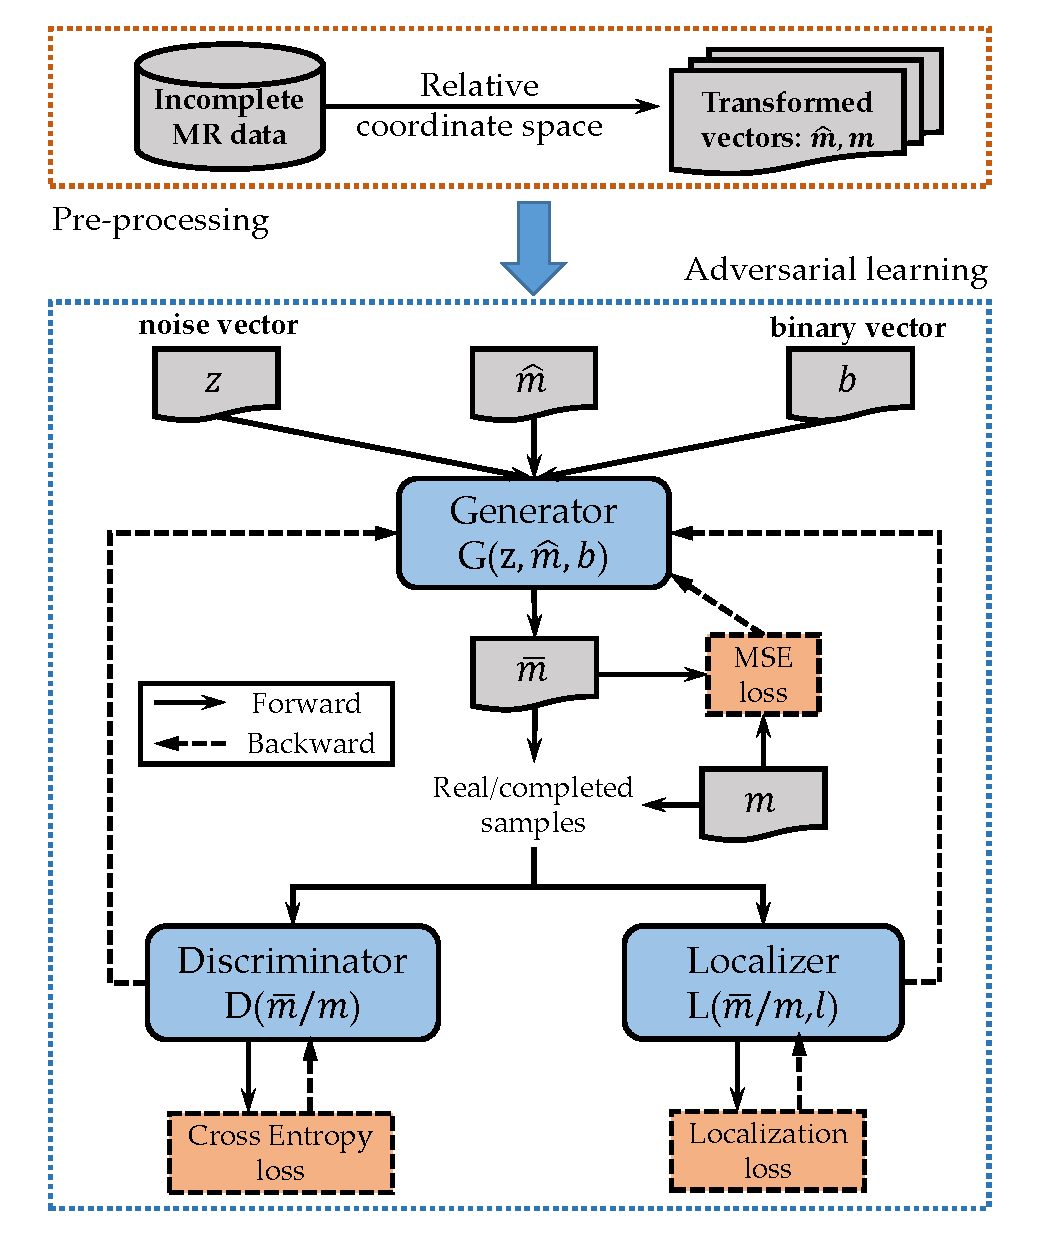
\includegraphics[width=9cm]{pics/framework.pdf}
  \caption{The framework of TelcoGAN}\label{fig:framework}
\end{figure}


\subsection{Overview of TelcoGAN}
The TelcoGAN model consists of pre-processing step and three basic components. The framework of TelcoGAN is illustrated as Fig. \ref{fig:framework}.

In the pre-processing step, due to sparse extensive cell locations in MR data, we propose to apply a serving-centric space. Then the sparse global coordinate-based distribution of MR data is transformed into a dense relative coordinate-based distribution. Thus TelcoGAN model can better capture the internal correlation of MR data.

The adversarial learning step consists of three interacting components described as follows:

(1) \textbf{Generator} $\bar{\textbf{m}}\sim$ G(\textbf{z},$\hat{\textbf{m}}$, \textbf{b}): The generator takes a random vector, an incomplete MR matrix and corresponding binary vector as input, and generates a completed MR matrix $\bar{\textbf{m}}$ that fools the discriminator as well as makes localizer produce accurate predictions.

(2) \textbf{Discriminator} D($\bar{\textbf{m}}/\textbf{m}$): The discriminator takes either a complete MR sample or a real MR sample as input, and gives each sample the probability over two categories (real/completed).

(3) \textbf{Localizer} L($\bar{\textbf{m}}/\textbf{m}$, $\textbf{l}$): The localizer takes a pair of MR sample and corresponding location label as input. It tries to predict the position of MR sample and minimize the localization loss.

The intuition of how our TelcoGAN model can generate high quality MR data for Telco localization is as follows. The generator tries to recover complete MR data samples based on observed variables to fool the discriminator; The discriminator distinguishes input data samples and computes probability distribution that the samples comes from real data or generated data; The localizer predicts locations of MR samples and produces a score for each sample that reflects its quality. During the adversarial game between the generator and the discriminator, the localizer can guide the optimization towards better data quality by utilizing available location labels. When the training reaches the optimality, the generator will have learnt the mapping from incomplete MR data to complete MR data.

We choose to implement these three components as neural networks. We will discuss their detailed structures for generating complete MR data in the following subsections.

\subsection{Serving-centric Space}
Here we construct a serving-centric space for MR data to better learn the internal relationship.

As seen in Table. \ref{tab:mr}, each MR record has a serving cell. According to Telco operations \cite{DBLP:conf/infocom/RayDM16}, the serving cell is selected from these nearby cells with good connection, which means close distance to mobile device. Thus a serving cell indicates a specific spatial domain. Given the total MR records with extensive global spatial domain, we group them as multiple local spatial domains by the serving cell. Then the whole city-scale area is divided into multiple small spatial domains.

Based on the division above, we propose a \emph{serving-centric space}, to transform the sparse global spatial distribution into a dense local one. In Fig. , a spatial domain is an area centered on the serving cell. Provided the cell tower database from Telco operators, we can obtain the GPS coordinate location of each cell. Based on the cell location data, we can do coordinate conversion as follows. Suppose the GPS coordinate (longitude, latitude) of the serving cell is $(x_0,y_0)$, those of the neighboring cells are $\{(x_i,y_i)\}$($1\leq i\leq 5$). Under the serving-centric space, the new coordinates are $(0,0)$ and $\{(x_i-x_0,y_i-y_0)\}$($1\leq i\leq 5$) for the serving cell and the neighboring cells respectively.

The \textbf{rational} behind serving-centric space is not difficult to understand: suppose normal cells and similar RF environment, in principle, the received signal strengths are only decided by the relative locations of connected cells and the MD. The serving-centric space offers advantages as: 1) reveal the true internal relationship of MR data and 2) knowledge learned from a domain can transfer to another domain and improve data quality.


\subsection{TelcoGAN Generator}
The goal here is to generate completed MR data by modelling the conditional probability of completed MR data given missing MR data.

The generator G takes a MR record $\hat{m}$ with missing RSSI, a random noise vector $z$ and an indicator vector $b$ as input, and outputs a complete MR record $\bar{m}$. The generator G is realized as convolutional neural networks (CNN), due to its capability of learning complex interactions. The process of generator G can be formulated by:

\begin{equation}\label{eq:gen}
  \tilde{m} = G(\hat{m}, (1-b)\odot z)
\end{equation}

where $\odot$ denotes element-wise multiplication. $(1-b)\odot z$ indicates random values to fill in missing RSSI in $\hat{m}$, that is, G uses random noise vector to replace the missingness for initialization of incomplete MR. Then G learns the conditional probability $P(\tilde{m}|\hat{m}, b, z)$ by convolutional nets.

\subsection{TelcoGAN Discriminator}
The TelcoGAN discriminator aims to differentiate completed MR records from the real ones by modelling the distribution of MR data.

The discriminator D takes either a completed MR record or a real MR record as input, and outputs the probability over two categories (real/completed). The D learns the probability of MR data $P(m)$ by full-convolution structure.

\subsection{TelcoGAN Localizer}


\subsection{TelcoGAN Training}

\section{Experiments}

\subsection{Data sets and Evaluation metrics}

\subsection{Counterparts}

\subsection{Baseline Experiment}

\subsection{TelcoGAN with Different Portions of Missing RSSI}

\subsection{Ablation Study}


\section{Related Work}

\textbf{Missing data completion}:
The pervasive missing data completion problem, also known as data imputation, has been extensively studied for many years. Generally, the data completion techniques are either discriminative or generative.

\textbf{Telco localization}:

\textbf{Deep learning and GANs}:
\section{Conclusion}

\newpage
\bibliographystyle{IEEEtran}
\bibliography{bib/reference,bib/localization,bib/imputation}

\end{document}
